\chapter{Multivariable derivatives} \label{multi}

In this chapter, we will study derivatives of functions $S \to \R^n$ where $S$ is a subset of $\R^m$. As it turns out, the most important case is when $n = 1$. In other words, the ``multi'' in the name of this chapter (as opposed to the ``single'' in the name of the previous chapter) is really referring to the fact that we might have $m > 1$ (rather than to the fact that we might have $n > 1$). Moreover,  the single variable case is actually quite important for the multivariable case; we'll often use results from \cref{single} to prove their multivariable counterparts. 

We'll begin by analyzing a particular example to build up some geometric intuition in \cref{multi-introductory-example}, and then proceed with the abstract discussion of multivariable derivatives. 

\section{Example} \label{multi-introductory-example}

Recall that we started off our discussion of single variable derivatives starting with a very geometric idea of tangent lines to graphs. For large values of $m$ (and $n$), graphs become hard to visualize and it is not so clear what ``tangent'' should mean. But there is at least one multivariable situation where, by exerting some strain on the three-dimensional visualization sectors of our brain, we can geometrically formalize what ``tangent'' might mean. This is the $m = 2, n = 1$ situation. The graph of such a function is a surface in $\R^3$, and its ``tangent'' at a point should be a plane. 

By analyzing a specific function $f : \R^2 \to \R$,  we can get some valuable insights into multivariable derivatives; the analysis will presage many of the concepts we will discuss later in the chapter. Any function would do, but let's focus on the function $f : \R^2 \to \R$ defined by
\[ f(x, y) = x^2 + y^2 \]
for our analysis.  

\subsection*{Describing the graph of \texorpdfstring{$f$}{f}}

First off, let's try to get a solid understanding of the graph of $f$. The graph $\Gamma$ is a subset of $\R^2 \times \R = \R^3$ defined by
\[ \Gamma = \{ (x, y, z) : z = f(x, y) \} = \{ (x, y, z) : z = x^2  + y^2 \}. \]
To visualize $\Gamma$, we will repeatedly slice $\Gamma$ along various planes. 

If we consider the slice obtained by setting $x = 0$, we find a parabola $z = y^2$. Similarly, if we consider the slice obtained by setting $x = 1$, we obtain the parabola $z = 1 + y^2$. Fixing $x = 5$, we obtain the parabola $z = 25 + y^2$. In fact, we can see that no matter what value of $x$ we fix, the resulting slice is always a parabola, just translated up from the origin by differing amounts (that amount being $x^2$). 

It's also worth considering the ``level sets,'' which are the slices of $\Gamma$ obtained by fixing various values of $z$. When $z = 0$, there is just the single point $x = y = 0$, ie, the origin. Fixing $z = 1$, the slice is given by $1 = x^2 +  y^2$, which is a circle of radius 1. Fixing $z = 17$, the slice is $17 = x^2 + y^2$, which is circle of radius $\sqrt{17}$. In fact, all of the level sets are circles. 

Putting these slices together, we see that the graph $\Gamma$ is a ``big parabolic bowl.''

\subsection*{Tangent plane at \texorpdfstring{$a = (2,1)$}{a = (2,1)}}

Now that we understand what the graph of $f$ looks like, let's try to figure out what the ``tangent plane'' $T$ at a point $a = (2,1)$ will look like. Of course, it's a plane inside $\R^3$ that passes through the point $(2, 1, f(2,1)) = (2, 1, 5)$. To specify which plane it actually is, we start by describing some lines that lie on this plane. 

Consider the $y = 1$ slice. We know that the graph of $\Gamma$ along this slice is the parabola $z = x^2 + 1$. So, slicing the tangent plane $T$ along $y = 1$ should yield the tangent line to this function of one variable, which we know how to compute from \cref{single}. The slope of this tangent line is
\[ \left.\frac{d }{d x} f(x, 1) \right|_{x = 2} = 4. \]
This quantity is called a \emph{partial derivative of $f$}, and will be denoted $(\partial f/\partial x)(a)$.  Thus the tangent line is the line parametrized by
\[ h \mapsto (2,1,5) + h \cdot (1, 0, 4). \]
Similarly, we can consider the $x = 2$ slice. We know that the graph $\Gamma$ along this slice is the parabola $z = 4 + y^2$.The slope of the corresponding tangent line is
\[ \frac{\partial f}{\partial y}(a) = \left.\frac{d f(2, y)}{dy}\right|_{y = 1} = 2. \]
Thus this tangent line is the line parametrized by
\[ k \mapsto (2,1,5) + k \cdot (0,1,2). \]

These two lines must uniquely determine the entire plane $T$. One way of describing $T$ that immediately falls out of the parametrizations we've found of the tangent lines is the plane parametrized by
\[ \begin{bmatrix} h \\ k \end{bmatrix} \mapsto \begin{bmatrix} 2 \\ 1 \\ 5 \end{bmatrix} + \begin{bmatrix} h \\ k \\ 4h + 2k \end{bmatrix}. \]
The important part of this expression is the bottom entry on the far right, the $4h + 2k$. To see why, consider the function $\R^2 \to \R$ given by $(h, k)  \mapsto 4h + 2k$. This is what we will call the \emph{(total) derivative} of $f$ and denote by $df_a$. Notice that $df_a$ is a linear map $\R^2 \to \R$. Moreover, its graph is a plane passing through the origin that is parallel to $T$. In other words, if we take the graph of $df_a$ and translate it over to the point $(2,1,5)$, we obtain exactly the tangent plane $T$. Speaking more loosely, the derivative $df_a : \R^2 \to \R$ records all of the ``slopey information'' about the tangent plane $T$. 

Notice moreover that, if $e_1, e_2$ are the standard basis vectors of $\R^2$ (cf. \cref{euclidean}), then
\[ \begin{aligned} df_a(e_1) &= 4 = \frac{\partial f}{\partial x}(a) \\
df_a(e_2) &= 2 = \frac{\partial f}{\partial y}(a) \end{aligned} \]
so the standard matrix representation $[df_a]$ (cf. \cref{matrix-representation-standard}) of the linear map $df_a$ is \begin{equation} \label{jacobian-matrix-example} [df_a] = \begin{bmatrix} 4 & 2 \end{bmatrix} = \begin{bmatrix} \dfrac{\partial f}{\partial x}(a) & \dfrac{\partial f}{\partial y}(a) \end{bmatrix}. \end{equation}

\subsection*{\texorpdfstring{$df_a$}{dfa} as an approximation}

Consider the function $\epsilon : \R^2 \to \R$ defined by
\[ v \mapsto |f(a+v)-f(a)-df_a(v)|.  \]
If $v = (h, k)$, we have
\[ \epsilon(v) = \epsilon\left( \begin{bmatrix} h \\ k \end{bmatrix} \right) \mapsto |(2+h)^2 + (1+k)^2 - 5 - 4h - 2k| = |h^2 + k^2| = \left|\begin{bmatrix} h \\ k \end{bmatrix} \right|^2 = |v|^2. \]
Notice that $\epsilon$ gets small rapidly as $v \to 0$. More precisely, notice that
\[ \lim_{v \to 0} \frac{\epsilon(v)}{|v|} = \lim_{v \to 0} |v| = 0, \]
so $\epsilon = o(|v|)$ as $v \to 0$. Since $\epsilon$ gets small rapidly, we can say that the function $v \mapsto f(a) + df_a(v)$ is a good approximation of the function $v \mapsto f(a+v)$ for small values of $v$. Said differently, letting $x = a + v$, the function $x \mapsto f(a) + df_a(x-a)$ is a good approximation of $f$ near $a$. 

\subsection{Overview}

In what follows, we will turn the above example on its head and \emph{define} the derivative using approximations. In other words, the derivative $df_a$ will be defined to be a linear function which yields a good approximation of $f$ near a point $a$. Then we will prove in \cref{jacobian-matrix} that the partial derivatives can be used to compute the standard matrix representation $df_a$, as we noted in \cref{jacobian-matrix-example} above. 

This might seem a bit ``backwards,'' given our analysis of the example above, but there is a good reason for doing this; it turns out that there are some bizarre functions where partial derivatives make sense, but tangent planes do not (cf. \cref{partials-dont-imply-differentiable} below).

As you may be able to tell, we'll be using linear algebra heavily in this chapter. We'll also need some facts about the operator norm; I encourage you to at least skim through \cref{operator-norm-basic}. 

\section{Definition of the derivative}

Throughout, $S$ will denote a subset of $\R^m$. 

\begin{definition}[Differentiability at a point] \index{differentiable!differentiable at a point}
	A function $f : S \to \R^n$ is \emph{differentiable at} an interior point $a \in S$ if there exists a linear map $\ell : \R^m \to \R^n$ such that
	\[ |f(a+h)-f(a)-\ell(h)| = o(|h|) \text{ as } h \to 0. \]
\end{definition}

It turns out that there can exist at most one linear map that has the above property. 

\begin{lemma} \label{differential-unique}
	Suppose $f : S \to \R^m$ is differentiable at an interior point $a \in S$. If $\ell$ and $\ell'$ are both linear maps $\R^m \to \R^n$ such that
	\[ |f(a+h) - f(a) - \ell(h)| = o(|h|) \text { and } |f(a+h) - f(a) - \ell'(h)| = o(|h|) \text{ as } h \to 0, \]
	then $\ell = \ell'$. 
\end{lemma}

\begin{proof}
	Let $\phi = \ell' - \ell$. Then $\phi$ is also a linear map $\R^m \to \R^n$. Moreover, observe that
	\[ \begin{aligned} |\phi(h)| &= |\ell'(h) - \ell(h)| \\
	&= |(f(a+h)-f(a)-\ell(h))-(f(a+h)-f(a)-\ell'(h)| \\
	&\leq |f(a+h)-f(a)-\ell(h)| + |f(a+h)-f(a)-\ell'(h)|. \end{aligned} \]
	Since both $|f(a+h)-f(a)-\ell(h)|$ and $|f(a+h)-f(a)-\ell'(h)|$ are $o(|h|)$, \cref{less-than-small-is-small,little-o-vector-space} imply that $|\phi(h)| = o(|h|)$ also. Then \cref{linear-and-small} implies that $\phi = 0$. 
\end{proof}

\begin{exercise}
	Look at the exercises from \cref{prelims} that are invoked in the proof above (namely, \cref{less-than-small-is-small,little-o-vector-space,operator-norm-is-norm}) and do any of them that you haven't already done.
\end{exercise}

\Cref{differential-unique} guarantees that the following definition makes sense.  

\begin{definition}[Derivative at a point] \index{derivative!derivative at a point} \index{total derivative|see {derivative}} \index{differential|see {derivative}}
	Suppose $f : S \to \R^n$ is differentiable at an interior point $a \in S$. Then the \emph{derivative of $f$ at $a$}, denoted $df_a$, is the unique linear map $\R^m \to \R^n$ satisfying
	\[ |f(a+v)-f(a)-df_a(h)| = o(|h|) \text{ as } h \to 0.  \]
	Sometimes $df_a$ is also called the \emph{total derivative} or the \emph{differential} of $f$ at $a$. 
\end{definition}

We've now defined the derivative, but it's fairly difficult to use this definition in practice. There are very few examples that can be computed directly from the definition. Here are some.

\begin{exercise} \label{derivative-of-linear}
	Suppose $\ell : \R^m \to \R^n$ is a linear map. Prove that $d\ell_a = \ell$ for all $a \in \R^m$.  
\end{exercise}

\begin{exercise} \label{derivative-of-multiplication}
	Let $\mu : \R^2 \to \R$ be the multiplication map $\mu(x, y) = xy$. Use the definition of the derivative to prove that
	\[ d\mu_{(a,b)}(h, k) = bh + ak \]
	for all $(a,b) \in \R^2$ and $(h,k) \in \R^2$. 
\end{exercise}

\begin{exercise} \label{derivative-of-line}
	Suppose $v, w \in \R^n$ and $f : \R \to \R^n$ is given by $f(t) = v + tw$. Calculate $df_a$ for any $a \in \R$. What is $df_a(1)$?
\end{exercise}

We will develop a bit more theory in order to compute derivatives more easily. Meanwhile, we can prove the following directly from the definition. 

\begin{exercise} \label{differentiable-implies-continuous}
	If $f : S \to \R^n$ is differentiable at an interior point $a \in S$, show that $f$ must be continuous at $a$. 
\end{exercise}

\section{Computing derivatives}

\subsection{Sum and scalar multiples rule} 

\begin{exercise}[Sum rule] \label{sum-rule} \index{sum rule}
	Prove that, if $f, g : S \to \R^n$ are both differentiable at an interior point $a \in S$, then $f + g$ is also differentiable at $a$ and \[ d(f+g)_a = df_a + dg_a. \]
\end{exercise}

\begin{exercise}[Scalar multiples rule] \label{scalar-multiples-rule} \index{scalar multiples rule}
	Prove that, if $c$ is a constant and $f : S \to \R^n$ is differentiable at an interior point $a \in S$, then $cf$ is also differentiable at $a$ and \[ d(cf)_a = c \cdot df_a. \]
\end{exercise}

\subsection{Chain rule}

The proof of the following is essentially the same as the second proof of the single variable chain rule given in \cref{chain-rule-single-section}. Since this proof is basically a repeat, some details are omitted; you are asked to fill in the details in \cref{chain-rule-details} below. 

\begin{theorem}[Chain rule] \label{chain-rule} \index{chain rule}
	Suppose that $S$ and $T$ are subsets of $\R^m$ and $\R^n$, respectively, that $f : S \to \R^n$ is differentiable at an interior point $a$, that $f(S) \subseteq T$ and $f(a)$ is an interior point of $T$, and that $g : T \to \R^p$ is differentiable at $f(a)$. Then the composite $g \circ f : S \to \R^p$ is also differentiable at $a$, and 
	\[ d(g \circ f)_a = dg_{f(a)} \circ df_a. \]
\end{theorem}

\begin{proof}
	Define the ``error in approximation'' functions\index{error in approximation function@``error in approximation'' function}
	\[ \begin{aligned} 
	r(h) &= f(a+h)-f(a) - df_a(h) \\ 
	s(k) &= g(f(a)+k)-g(f(a))-dg_{f(a)}(k) 
	\end{aligned} \]
	and then observe that
	\begin{equation} \label{rewrite-error} g(f(a+h)) - g(f(a)) - dg_{f(a)}(df_a(h)) = dg_{f(a)}(r(h)) + s(df_a(h)+r(h)). \end{equation}
	This means that 
	\[ |g(f(a+h)) - g(f(a)) - dg_{f(a)}(df_a(h))| \leq |dg_{f(a)}(r(h))| + |s(df_a(h)+r(h))|. \]
	Since $dg_{f(a)}$ is linear and $|r(h)| = o(|h|)$, \cref{chain-rule-details} guarantees that $|dg_{f(a)}(r(h))| = o(|h|)$ also. Thus, by \cref{little-o-vector-space}, it is sufficient to prove that $|s(df_a(h) + r(h))| = o(|h|)$. To do this, define $\eta(k) = |s(k)|/|k|$ and then notice that 
	\[ \begin{aligned} \frac{|s(df_a(h)+r(h))|}{|h|} &= \eta(df_a(h)+r(h)) \cdot \frac{|df_a(h) + r(h)|}{|h|} \\
	&\leq \eta(df_a(h) + r(h)) \left( \|df_a\| + \frac{|r(h)|}{|h|} \right). \end{aligned} \]
	We now take the limit as $h \to 0$. Using the facts that $\eta \circ (df_a + r)$ is continuous at 0 and that $|r(h)| = o(|h|)$, we obtain the result. 
\end{proof}

\begin{exercise} \label{chain-rule-details}
	\begin{enumerate}[(a)]
		\item Prove \cref{rewrite-error}. 
		\item \label{linear-of-small-is-small} Suppose $r : \R^m \to \R^n$ is a function such that $|r(h)| = o(|h|)$ as $h \to 0$. If $\ell : \R^n \to \R^p$ is linear, prove that $|\ell(r(h))| = o(|h|)$ also.
		
		\begin{hint} Even though the operator norm\index{operator norm} does not appear anywhere in the statement of this exercise, you might find the concept useful. In particular, you might consider doing \cref{operator-norm-reformulation} and then using it to prove (\ref{linear-of-small-is-small}). 
		\end{hint}
		
		\item Prove that $\eta \circ (df_a + r)$ is continuous at 0. 
	\end{enumerate}
\end{exercise}

\begin{comment}
\begin{proof}
Observe that
\[ \frac{|\ell(r(v))|}{|v|} \leq \frac{\|\ell\| \cdot |r(v)|}{|v|}. \]
Since $|r(v)| = o(|v|)$, we see that the right-hand side tends to 0 as $v \to 0$. The squeeze theorem thus guarantees that $|\ell(r(v))| = o(|v|)$ also. 
\end{proof}
\end{comment}

\subsection{Differentiability by components}

Recall that we asserted at the beginning of this chapter that the ``multi'' in the name of this chapter refers to the number of inputs (rather than the number of outputs). This section is where we show that understanding the $n = 1$ case is ``enough'' to understand general $n$.

\begin{definition}[Component functions] \index{component function}
	For any function $f : S \to \R^n$, we define the $j$th \emph{component function} $f_j : S \to \R$ to be the composite $\pi_j \circ f$, where $\pi_j$ is the $j$th projection map (cf. \cref{euclidean}).\index{projection map}
\end{definition}

\begin{proposition} \label{differentiable-by-components}
	A function $f : S \to \R^n$ is differentiable at an interior point $a \in S$ if and only if the component function $f_j : S \to \R$ is differentiable at $a$ for all $j = 1, \dotsc n$. Moreover,
	\begin{equation} \label{derivative-of-components} df_a(h) = \begin{bmatrix} df_{1,a}(h) \\ \vdots \\ df_{n,a}(h) \end{bmatrix}. \end{equation}
\end{proposition}

\begin{proof}
	If $f$ is differentiable at $a$, then the composite $f_j = \pi_j \circ f$ is also differentiable at $a$ by the chain rule \ref{chain-rule}. Moreover, since $\pi_j$ is linear, we know that $d\pi_{j,f(a)} = \pi_j$ by \cref{derivative-of-linear}. Thus, by the chain rule, 
	\[ df_{j,a}(h) = (d\pi_{j,f(a)} \circ df_a)(h) = \pi_j(df_a(h)) \]
	for all $j$, which is precisely \cref{derivative-of-components}. 
	For the converse, we turn \cref{derivative-of-components} on its head. Suppose $f_j$ is differentiable at $a$ for all $j$, and let $\ell : \R^m \to \R^n$ be the linear map 
	\[ \ell(h) = \begin{bmatrix} df_{1,a}(h) \\ \vdots \\ df_{n,a}(h) \end{bmatrix}.  \]
	We now want to show that $|f(a+h)-f(a)-\ell(h)| = o(|h|)$ as $h \to 0$. Observe that the component functions of $h \mapsto f(a+h)-f(a)-\ell(h)$ are given by
	\[ v \mapsto \pi_j \left( f(a+h)-f(a)-\ell(h) \right) = f_j(a+h)-f_j(a)-df_{j,a}(h) \]
	since $\pi_j$ is linear, 
	and we know that $|f_j(a+h)-f_j(a)-df_{j,a}(h)| = o(|h|)$. By \cref{components-are-small-implies-small} below applied with the function $r(h) = f(a+h)-f(a)-\ell(h)$, we conclude that $|f(a+h)-f(a)-\ell(h)| = o(|h|)$. 
\end{proof}

\begin{exercise} \label{components-are-small-implies-small}
	Show that if $S$ is a neighborhood of 0 in $\R^m$ and $r :  S  \to \R^n$ is a function such that $|r_j(h)| = o(|h|)$ as $h \to 0$ for all $j = 1, \dotsc, n$, then $|r(h)| = o(|h|)$ also.
	\begin{hint}
		You may find it useful to do \cref{max-l2} first. 
	\end{hint}
\end{exercise}

\subsection{Product and quotient rules}

We showed in the previous section that it's enough to understand the $n = 1$ case. So in this section and the next, we'll focus our attention on the $n = 1$ case and try to understand this better. Note that, when $n = 1$, we have more operations available to us; we can multiply and divide such functions. 

So let's start off by establishing product and quotient rules. As it turns out, we can actually derive these using the multivariable chain rule \ref{chain-rule}!

\begin{proposition}[Product rule] \label{product-rule} \index{product rule}
	Suppose $f, g : S \to \R$ are both differentiable at an interior point $a \in S$. Then $fg$ is also differentiable at $a$ and
	\[ d(fg)_a = g(a)df_a + f(a) dg_a. \]
\end{proposition}

\begin{proof}
	Let $f \times g$ denote the function $S \to \R^2$ defined by
	\[ (f \times g)(x) = (f(x), g(x)). \]
	Observe that the first and second component functions of $f \times g$ are $f$ and $g$, respectively; thus it follows from \cref{differentiable-by-components} that 
	\[ d(f \times g)_a(h) = (df_a(h), dg_a(h)). \]
	Let $\mu : \R^2 \to \R$ denote the multiplication map $\mu(x,y) = xy$ that we considered in \cref{derivative-of-multiplication}. Then $fg = \mu \circ (f \times g)$, so by the chain rule \ref{chain-rule}, we have that 
	\[ \begin{aligned} d(fg)_a(h) &= d\mu_{(f(a),g(a))}(d(f \times g)_a(h)) \\
	&= d\mu_{f(a),g(a)}(df_a(h), dg_a(h)) \\
	&= g(a) df_a(h) + f(a)dg_a(h), \end{aligned} \]
	where we have used the calculation from \cref{derivative-of-multiplication} for the final step. 
\end{proof}

\begin{exercise} \label{one-over-rule}
	Suppose $f : S \to \R$ is differentiable at an interior point $a \in S$ and that $f(a) \neq 0$. Show that $1/f$ is also differentiable at $a$, and
	\[ d(1/f)_a = -\frac{df_a}{f(a)^2}.  \]
	\begin{hint}
		Consider the function $\iota : \R \setminus \{0\} \to \R$ given by $\iota(x) = 1/x$. This is a single variable function, so we know $d\iota_x$ from \cref{single}. Now note that $1/f = \iota \circ f$. 
	\end{hint}
\end{exercise}

\begin{exercise}[Quotient rule] \label{quotient-rule} \index{quotient rule}
	Suppose $f, g : S \to \R$ is differentiable at an interior point $a \in S$ and that $g(a) \neq 0$. Show that $f/g$ is also differentiable at $a$, and that
	\[ d(f/g)_a = \frac{g(a)df_a - f(a)dg_a}{g(a)^2}. \]
	\begin{hint}
		Combine \cref{one-over-rule,product-rule}. 
	\end{hint}
\end{exercise}

\subsection{Partial derivatives}

\begin{definition}[Partial derivatives] \index{partial derivative}
	Suppose $f : S \to \R$ is a function and $a \in S$ is an interior point. The \emph{$i$th partial derivative of $f$ at $a$}, denoted $\partial_i f(a)$, is defined to be the limit
	\[ \lim_{s \to 0} \frac{f(a+se_i) - f(a)}{s}, \]
	where $e_i$ denotes the $i$th standard basis vector (cf. \cref{euclidean}). If we're using $x$ to denote the input to $f$ and $x_i$ to denote the $i$th component of the input, $\partial_i f(a)$ is sometimes also denoted by one of the following. 
	\[ f_{x_i}(a) \quad \left. \frac{\partial f}{\partial x_i}\right|_{x = a} \quad \left.\frac{\partial}{\partial x_i} f(x)\right|_{x = a} \quad \frac{\partial f}{\partial x_i}(a) \]
\end{definition}

You may remember from multivariable calculus that partial derivatives behave a great deal like single variable derivatives. The reason for this is the following important remark, which reinterprets the partial derivative as a single variable derivative. 

\begin{remark} \label{partial-to-single}
	Consider the function $\xi_i : \R \to \R^m$ given by $\xi_i(s) = a + se_i$. Then 0 is an interior point of $T = \xi_i^{-1}(S) \subseteq \R$, and $f \circ \xi_i$ is a single variable function $T \to \R$. Moreover, we have
	\[ \partial_i f(a) = (f \circ \xi_i)'(0), \]
	just by writing out the definition of both sides. 
\end{remark}

\begin{example} \label{computing-partials-example}
	Consider the function $f : \R^2 \to \R$ given by $f(x, y) = \sin(xy^2)$. Fix $(a, b) \in \R^2$ and define $\xi : \R \to \R^2$ by $\xi(s) = (a + s, b)$, as in \cref{partial-to-single}. Then
	\[ (f \circ \xi)(s) = f(a + s, b) = \sin((a+s)b^2).  \]
	Then
	\[ \begin{aligned} \frac{\partial f}{\partial x}(a, b) &= (f \circ \xi)'(0) \\
	&= \left.\frac{d}{ds} \left(\sin((a+s)b^2) \right) \right|_{s = 0} \\
	&= \left. b^2\cos((a+s)b^2)\right|_{s = 0} \\
	&= b^2\cos(ab^2). \end{aligned}  \]
\end{example}

\begin{exercise}
	With notation as in \cref{computing-partials-example}, compute $(\partial f/\partial y)(a, b)$. 
\end{exercise}

We can also use \cref{partial-to-single} to prove some partial derivative analogs of results we proved in \cref{single}.

\begin{exercise}[Product rule for partial derivatives] \label{product-rule-partials} \index{product rule}
	Suppose $f, g : S \to \R$ are functions and $a \in S$ is an interior point such that $\partial_i f(a)$ and $\partial_i g(a)$ both exist. Prove that $\partial_i (fg)(a)$ also exists and that
	\[ \partial_i (fg)(a) = g(a)\partial_i(f)(a) + f(a) \partial_i g(a). \]
	\begin{hint} Use \cref{partial-to-single} and the single variable product rule \ref{product-rule-single}. \end{hint}
\end{exercise}

\begin{exercise}[Quotient rule for partial derivatives] \label{quotient-rule-partials} \index{quotient rule}
	Suppose $f, g : S \to \R$ are functions and $a \in S$ is an interior point such that $g(a) \neq 0$ and $\partial_i f(a)$ and $\partial_i g(a)$ both exist. Show that $\partial_i(f/g)(a)$ also exists and 
	\[ \partial_i(f/g)(a) = \frac{g(a)\partial_i f(a) - f(a)\partial_i g(a)}{g(a)^2}. \]
	\begin{hint} Use \cref{partial-to-single} and the single variable quotient rule \ref{quotient-rule-single}. \end{hint} 
\end{exercise}

\begin{exercise}[Interior extremum theorem for partial derivatives] \label{interior-extremum-partials} \index{extremum!interior extremum theorem}
	Suppose $f : S \to \R$ is a function and an interior point $a \in S$ is a local extremum of $f$. Show that, if $\partial_i f(a)$ exists, then $\partial_i f(a) = 0$. \begin{hint} Use \cref{partial-to-single} and the single variable interior extremum theorem \ref{interior-extremum}. \end{hint}
\end{exercise}

As we noted in \cref{single}, the single variable interior extremum theorem \ref{interior-extremum} is false (cf. \cref{interior-extremum-converse-false}). The same is true for the interior extremum theorem for partial derivatives \ref{interior-extremum-partials}, except that there are now even more ways for the converse to fail. Here are two examples to illustrate this.  

\begin{example}
	Consider the function $f : \R^2 \to \R$ given by \[ f(x, y) = x^2 - y^2. \]
	Let $\xi(s) = 0 + se_1 = (s, 0)$ and $\eta(s) = 0 + se_2 = (0, s)$. Then $f \circ \xi$ has a minimum at 0, so $(f \circ \xi)'(0) = (\partial f)/(\partial x)(0) = 0$. Similarly, $f \circ \eta$ has a maximum at 0, so $(f \circ \eta)'(0) = (\partial f)/(\partial y)(0) = 0$ also. But clearly these two facts together mean that 0 cannot be a local extremum of $f$. 
	
	% TODO: picture
\end{example}

\begin{exercise}
	Consider the function $f : \R^2 \to \R$ given by 
	\[ f(x, y) = (y- x^2)(y - 3x^2). \]
	\begin{enumerate}[(a)]
		\item Show that the origin is \emph{not} a local extremum of $f$. \begin{hint} Consider the values of $f$ on points of the form $(0,b)$ and $(a, 2a^2)$ near the origin. \end{hint}
		\item Show that $f$ restricted to the $x$-axis does have an absolute minimum at the origin. 
		\item Show that $f$ restricted to the $y$-axis also has an absolute minimum at the origin. 
		\item Show that $f$ restricted to an arbitrary line through the origin has an absolute minimum at the origin.
	\end{enumerate}

	% TODO: picture
\end{exercise}

Now for the main result of this section: partial derivatives is that they help us compute derivatives. Note that we will generalize this result in \cref{jacobian-matrix} below. 

\begin{proposition} \label{differentiable-implies-partials}
	If $f : S \to \R$ is differentiable at an interior point $a \in S$, then the $i$th partial derivative $\partial_i f(a)$ exists for all $i = 1, \dotsc m$, and the standard matrix representation $[df_a]$ of the linear map $df_a : \R^m \to \R$ is a $1 \times m$ matrix whose $i$th entry is $\partial_i f(a)$. 
	\[ [df_a] = \begin{bmatrix} \partial_1 f(a) & \partial_2 f(a) & \dotsb & \partial_m f(a) \end{bmatrix} \]
\end{proposition}

\begin{proof}
	Let $r$ be the ``error in approximation'' function
	\[ r(h) = f(a+h) - f(a) - df_a(h), \]
	so that $|r(h)| = o(|h|)$ as $h \to 0$. Letting $h = se_i$, we see that
	\[ r(se_i) = f(a+se_i) - f(a) - df_a(se_i) = f(a+se_i) - f(a) - s df_a(e_i) \]
	by linearity of $df_a$, so
	\[ \frac{r(se_i)}{s} = \frac{f(a+se_i) - f(a) - sdf_a(e_i)}{s} = \frac{f(a+se_i) - f(a)}{s} - df_a(e_i). \]
	Then 
	\[ \begin{aligned} \lim_{s \to 0} \left| \frac{f(a+se_i) - f(a)}{s} - df_a(e_i) \right| &= \lim_{s \to 0} \left| \frac{r(se_i)}{s} \right| \\&= \lim_{s \to 0} \frac{|r(se_i)|}{|s|} \\
	&= \lim_{s \to 0} \frac{|r(se_i)|}{|se_i|} \\
	&= 0 \end{aligned} \]
	where we used the fact that $|r(h)| = o(|h|)$ as $h \to 0$ for the final step. This tells us that
	\[ \partial_i f(a) = \lim_{s \to 0} \frac{f(a+se_i) - f(a)}{s} \]
	exists and equals $df_a(e_i)$. 
\end{proof}

\begin{remark} \label{gradient}
	If $f : S \to \R$ is differentiable at an interior point $a \in S$, then the vector \[ [df_a]^T = \begin{bmatrix} \partial_1 f(a) \\ \partial_2 f(a) \\ \vdots \\ \partial_m f(a) \end{bmatrix} \in \R^m \]
	is often called the \emph{gradient} of $f$ at $a$, and is denoted $\nabla f(a)$.\index{gradient} 
\end{remark}

Now for the important caveat: unfortunately, the converse to \cref{differentiable-implies-partials} is \emph{not} true. 

\begin{exercise} \label{partials-dont-imply-differentiable}
	Consider the function $f : \R^2 \to \R$ defined as follows.
	\[ f(x, y) = \begin{cases} \dfrac{x y}{x^2 + y^2} &  \text{if } (x, y) \neq 0 \\ 0 & \text{if } (x, y) = 0 \end{cases} \]
	Show that the partial derivatives of $f$ exist at the origin, but that $f$ is not even continuous at the origin (so it cannot be differentiable, by \cref{differentiable-implies-continuous}). \begin{hint} Approach the origin along the line $x = y$. \end{hint}
\end{exercise}

Thankfully, this phenomenon is fairly pathological; \cref{continuous-partials} will provide a converse to \cref{differentiable-implies-partials} under fairly mild additional hypotheses. 

\subsection{Jacobian matrix}

\begin{definition}[Jacobian matrix]  \index{jacobian matrix}
	Suppose $f : S \to \R^n$ is differentiable at an interior point $a \in S$. The \emph{Jacobian matrix} of $f$ at $a$, denoted $f'(a)$, is the $n \times m$ matrix whose $(j, i)$-entry is $\partial_i f_j(a)$. In other words,
	\[ f'(a) = \begin{bmatrix} \partial_1 f_1(a) & \partial_2 f_1(a) & \dotsb & \partial_m f_1(a) \\ 
	\partial_1 f_2(a) & \partial_2 f_2(a) & \dotsb & \partial_m f_2(a) \\
	\vdots & \vdots & \ddots & \vdots \\ 
	\partial_1 f_n(a) & \partial_2 f_n(a) & \dotsb & \partial_m f_n(a) \end{bmatrix} \]
	Note that \cref{differentiable-by-components,differentiable-implies-partials} tell us that all of these partial derivatives exist. 
\end{definition}

\begin{theorem} \label{jacobian-matrix}
	If $f : S \to \R^m$ is differentiable at an interior point $a \in S$, then $[df_a] = f'(a)$. 
\end{theorem}

\begin{exercise}
	Prove \cref{jacobian-matrix}. \begin{hint} Use \cref{differentiable-by-components,differentiable-implies-partials}. \end{hint}
\end{exercise}

Using \cref{jacobian-matrix}, many of the rules for differentiation we've seen acquire forms we may be more familiar with from single variable calculus. For example, since composition of linear maps corresponds to multiplication of the corresponding matrix representations, the chain rule \ref{chain-rule} states that 
\[ (g \circ f)'(a) = [d(g \circ f)_a] = [dg_{f(a)} \circ df_a] = [dg_{f(a)}] [df_a] = g'(f(a)) f'(a). \]
Though the equality $(g \circ f)'(a) = g'(f(a)) f'(a)$ looks superficially identical to the equality from the single variable chain rule \ref{chain-rule-single}, it's worth noticing that the terms in this multivariable version are \emph{matrices}. In particular, this means that that order of the multiplication $g'(f(a))f'(a)$ cannot be interchanged, whereas this was a non-issue in the single variable case. 

Similarly, the matrix version of the multivariable product rule \ref{product-rule} states that 
\[ (fg)'(a) = g(a)f'(a) + g(a)f'(a), \]
which again looks superficially identical to the single variable product rule \ref{product-rule-single}.  

\subsection{Rank of a differentiable map}

\begin{definition}[Rank of a differentiable map] \label{immersive-submersive-critical} \index{rank!of a differentiable function}
	Suppose $f : S \to \R^n$ is differentiable at an interior point $a \in S$. The rank of the linear map $df_a : \R^m \to \R^n$ is also called the \emph{rank of $f$ at $a$}, denoted $\rank_a(f)$. Note that $\rank_a(f) \leq \min\{m,n\}$.
	\begin{itemize}
		\item If $\rank_a(f) = m$, then we say that $f$ is \emph{immersive at $a$}.\index{immersive} Note that this is equivalent to asking that $df_a$ be injective. 
		\item If $\rank_a(f) = n$, then we say that $f$ is \emph{submersive at $a$}.\index{submersive} Note that this is equivalent to asking that $df_a$ be surjective. 
		\item If $\rank_a(f) = m = n$, then we say that $f$ is \emph{\'etale at $a$}.\index{etale@\'etale} Note that this is equivalent to asking that $df_a$ be an isomorphism. 
		\item If $\rank_a(f) = \min\{m,n\}$, then we say that $a$ is a \emph{regular point} of $f$.\index{regular point} 
		\item If $\rank_a(f) < \min\{m,n\}$, then we say that $a$ is a \emph{critical point} of $f$.\index{critical point}
	\end{itemize}
\end{definition}

There are lots of relationships between these notions, depending on how $m$ compares to $n$. You should convince yourself of the following facts.  
\begin{itemize}
	\item If $m > n$...
	\begin{itemize}
		\item $f$ cannot be immersive at any point.
		\item $a$ is a regular point of $f$ if and only if $f$ is submersive at $a$.
	\end{itemize}
	\item If $m < n$...
	\begin{itemize}
		\item $f$ cannot be submersive at any point.
		\item $a$ is a regular point of $f$ if and only if $f$ is immersive at $a$.
	\end{itemize}
	\item If $m = n$...
	\begin{itemize}
		\item $a$ is a regular point of $f$ if and only if $f$ is immersive at $a$, if and only if $f$ is submersive at $a$, if and only if $f$ is \'etale at $a$. 
	\end{itemize}
\end{itemize}

\begin{caution}
	A map $f$ being immersive or submersive at an interior point $a \in S$ is always defined as it is above, and critical points are always defined to be the opposite of regular points. But some mathematicians use a different definition of regularity: they define a point to be regular if $\rank_a(f) = n$, so that, by definition, it's \emph{always} true (for all $m, n$) that $f$ is a submersion at $a$ if and only if $a$ is a regular point of $f$. If $m \geq n$, there's no difference between these alternative definitions and our definitions. But, if $m < n$, there is a difference: these other mathematicians would say that all points are critical in this case, but that isn't true for us. So, if you see the words ``regular point'' and ``critical point'' in another text and it's possible that $m < n$, it's worth looking back to make sure you know what the author means!
\end{caution}

\begin{example} \label{polar-map}

Let $f : \R^2 \to \R^2$ be the map
\[ f(r,\theta) = (r\cos\theta, r\sin\theta). \]
See \cref{polar-map-picture}. 
\begin{figure}
	\begin{center}
		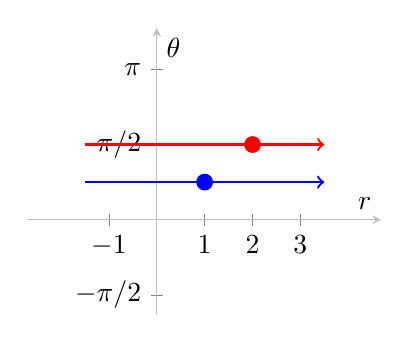
\begin{tikzpicture}
		\begin{axis}[
		xmin=-2,xmax=4,
		ymin=-2,ymax=4,
		ytick={-1.57,1.57,3.14},
		xtick={-1,1,2,3},
		yticklabels={$-\pi/2$,$\pi/2$, $\pi$},
		axis lines=middle,
		axis line style=lightgray,
		width=0.5\textwidth,
		xlabel={$r$},
		ylabel={$\theta$},
		axis equal
		] 
		
		\addplot[red,thick,->] expression[domain=-1.5:3.5,samples=2]{1.57};
		\node[color=red,draw=red,circle,fill,inner sep=2pt] at (axis cs:2,1.57) {}; 
		
		\addplot[blue,thick,->] expression[domain=-1.5:3.5,samples=2]{1.57/2};
		\node[color=blue,draw=blue,circle,fill,inner sep=2pt] at (axis cs:1,1.57/2) {}; 
		
		\end{axis}
		\end{tikzpicture}\hspace{1cm}
		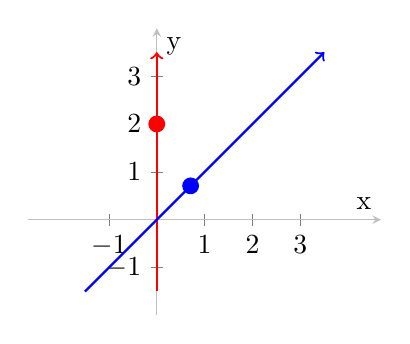
\begin{tikzpicture}
		\begin{axis}[
		xmin=-2,xmax=4,
		ymin=-2,ymax=4,
		ytick={-1,1,2,3},
		xtick={-1,1,2,3},
		axis lines=middle,
		axis line style=lightgray,
		width=0.5\textwidth,
		xlabel={x},
		ylabel={y},
		axis equal
		] 
		
		\addplot +[mark=none,red,thick,->] coordinates {(0, -1.5) (0, 3.5)};
		\node[color=red,draw=red,circle,fill,inner sep=2pt] at (axis cs:0,2) {}; 
		
		\addplot[blue,thick,->] expression[domain=-1.5:3.5,samples=2]{x};
		\node[color=blue,draw=blue,circle,fill,inner sep=2pt] at (axis cs:0.707,0.707) {}; 
		\end{axis}
		\end{tikzpicture}
		
		\mbox{}
		
		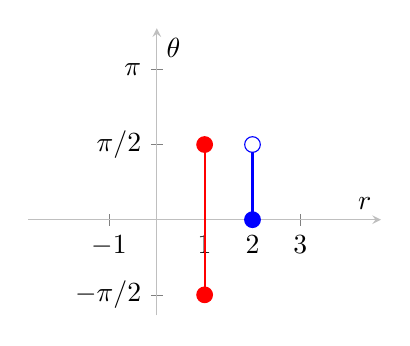
\begin{tikzpicture}
		\begin{axis}[
		xmin=-2,xmax=4,
		ymin=-2,ymax=4,
		ytick={-1.57,1.57,3.14},
		xtick={-1,1,2,3},
		yticklabels={$-\pi/2$,$\pi/2$, $\pi$},
		axis lines=middle,
		axis line style=lightgray,
		width=0.5\textwidth,
		xlabel={$r$},
		ylabel={$\theta$},
		axis equal
		] 
		
		\addplot +[mark=none,red,thick] coordinates {(1, -1.57) (1,1.57)};
		\node[color=red,draw=red,circle,fill,inner sep=2pt] at (axis cs:1,-1.57) {}; 
		\node[color=red,draw=red,circle,fill,inner sep=2pt] at (axis cs:1,1.57) {}; 
		
		\addplot +[mark=none,blue,thick] coordinates {(2, 0) (2,1.57)};
		\node[color=blue,draw=blue,circle,fill,inner sep=2pt] at (axis cs:2,0) {}; 
		\node[color=white,draw=blue,circle,fill,inner sep=2pt] at (axis cs:2,1.57) {}; 
		
		\end{axis}
		\end{tikzpicture}\hspace{1cm}
		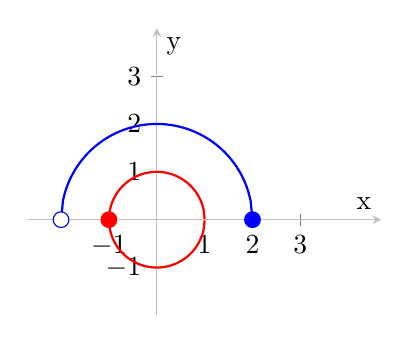
\begin{tikzpicture}
		\begin{axis}[
		xmin=-2,xmax=4,
		ymin=-2,ymax=4,
		ytick={-1,1,2,3},
		xtick={-1,1,2,3},
		axis lines=middle,
		axis line style=lightgray,
		width=0.5\textwidth,
		xlabel={x},
		ylabel={y},
		axis equal
		] 
		
		\addplot[red,thick] expression[domain=-1:1,samples=100]{sqrt(1-x^2)}; 
		\addplot[red,thick] expression[domain=-1:1,samples=100]{-sqrt(1-x^2)}; 
		\node[color=red,draw=red,circle,fill,inner sep=2pt] at (axis cs:-1,0) {}; 
		
		\addplot[blue,thick] expression[domain=-2:2,samples=100]{sqrt(4-x^2)}; 
		\node[color=blue,draw=blue,circle,fill,inner sep=2pt] at (axis cs:2,0) {}; 
		\node[color=white,draw=blue,circle,fill,inner sep=2pt] at (axis cs:-2,0) {}; 
		\end{axis}
		\end{tikzpicture}
	\end{center}
	\caption{The function $f(r, \theta) = (r\cos\theta, r\sin\theta)$ of \cref{polar-map} transforms the pictures on the right to the pictures on the left.}  \label{polar-map-picture}
\end{figure}
We compute partial derivatives. 
\[ \frac{\partial f_1}{\partial r} = \cos \theta \quad \frac{\partial f_2}{\partial r} = \sin \theta \quad \frac{\partial f_1}{\partial \theta} = -r\sin \theta \quad \frac{\partial f_2}{\partial \theta} = r\cos \theta.  \]
Thus
\[ f'(r, \theta) = \begin{bmatrix} \cos \theta & -r \sin \theta \\ \sin \theta & r \cos \theta \end{bmatrix}. \]
Since this is a square matrix, $df_{(r, \theta)}$ has non-maximal rank if and only if its determinant vanishes. But
\[ \det f'(r, \theta) = r\cos^2 \theta + r\sin^2 \theta = r, \]
so the critical locus\index{critical point!critical locus} (ie, the set of all critical points) of $f$ is the vertical line $r = 0$, and $f$ is \'etale away from this line. 
\end{example}

\begin{exercise} \label{cusp}
	Consider the function $f : \R \to \R^2$ defined by
	\[ f(x) = (x^2, x^3). \]
	See \cref{cusp-graph} for a picture of the image of $f$. 
	\begin{figure}
			\begin{center}
			\begin{tikzpicture}
			\begin{axis}[
			xmin=-0.5,xmax=2,
			ymin=-2,ymax=2,
			ytick={0},
			xtick={0},
			xticklabels={},
			yticklabels={},
			axis lines=middle,
			axis line style=lightgray,
			width=0.75\textwidth
			]
			\addplot[black,style=thick,->] expression[domain=0:1.5,samples=50]{ sqrt(x^3) };
			\addplot[black,style=thick,->] expression[domain=0:1.5,samples=50]{ -sqrt(x^3) }; 
			\node[color=black,draw=black,circle,fill,inner sep=2pt] at (axis cs:0,0) {}; 
			
			\end{axis}
			\end{tikzpicture}
		\end{center}
	\caption{The image of the function $f(x) = (x^2, x^3)$. The origin is $f(0)$.}  \label{cusp-graph}
	\end{figure}
	Calculate $f'(x)$ for all $x \in \R$. Then show that 0 is a critical point of $f$, and that $f$ is immersive away from 0.
	Loosely speaking, the fact that 0 is a critical point of $f$ corresponds geometrically to the fact that $f(0)$ is a ``pointy'' cusp\index{cusp}. 
\end{exercise}


\begin{exercise} \label{node}
	Consider the function $f : \R \to \R^2$ defined by
	\[ f(x) = (x^2-1, x^3-x). \]
	See \cref{node-graph} for a picture of the image of $f$. 
	\begin{figure}
		\begin{center}
			\begin{tikzpicture}
			\begin{axis}[
			xmin=-1.5,xmax=1,
			ymin=-1.5,ymax=1.5,
			ytick={0},
			xtick={},
			xticklabels={},
			yticklabels={},
			axis lines=middle,
			axis line style=lightgray,
			width=0.75\textwidth
			]
			\addplot[black,style=thick,->] expression[domain=-1:0.9,samples=500]{ sqrt(x^2*(x+1)) };
			\addplot[black,style=thick,->] expression[domain=-1:0.9,samples=500]{ - sqrt(x^2*(x+1)) }; 
			\node[label={$f(\pm1)$},color=black,draw=black,circle,fill,inner sep=2pt] at (axis cs:0,0) {}; 
			\node[label={120:$f(0)$},color=black,draw=black,circle,fill,inner sep=2pt] at (axis cs:-1,0) {}; 
			
			\end{axis}
			\end{tikzpicture}
		\end{center}
		\caption{The image of the function $f(x) = (x^2-1, x^3-x)$. We have $f(0) = (-1,0)$ and $f(\pm 1) = (0,0)$.}  \label{node-graph}
	\end{figure}
	Calculate $f'(x)$ for all $x \in \R$, and show that $f$ is immersive everywhere.
\end{exercise}

\begin{exercise}
	Show that an interior point $a \in S$ is a critical point\index{critical point} of $f : S \to \R$ if and only if $\partial_i f(a) = 0$ for all $i$. 
\end{exercise}

\section{Levels of differentiability}

Throughout this section, $U$ denotes an open subset of $\R^m$.

\subsection{Differentiable functions} 

\begin{definition}[Differentiability] \index{differentiable} \index{derivative}
	A function $f : U \to \R^n$ is \emph{differentiable} if it is differentiable at every $a \in U$. The \emph{derivative} of $f$, denoted $df$, is the function $U \to \mathscr{L}(\R^m, \R^n)$ given by $a \mapsto df_a$. Sometimes the function $df$ is also called the \emph{total derivative} or the \emph{differential} of $f$. 
\end{definition}

\begin{definition}
	If $f : U \to \R^n$ is differentiable, the \emph{$i$th partial derivative} of $f$, denoted $\partial_i f$, is the function $a \mapsto \partial_i f(a)$. If we're using $x$ to denote the input to $f$ and $x_i$ to denote the $i$th component of the input, $\partial_i f(a)$ is sometimes also denoted by one of the following. 
	\[ f_{x_i} \quad \frac{\partial f}{\partial x_i} \]
\end{definition}

Here is a multivariable generalization of \cref{constant-iff-derivative-zero-single}. In fact, we will use te single variable version to prove this multivariable version. 

\begin{proposition} \label{constant-iff-derivative-zero}
	Suppose $B$ is an open ball and $f : B \to \R^n$ is a differentiable function. Then $df = 0$ if and only if $f$ is constant\index{constant function}.  
\end{proposition}

\begin{proof}
	Taking $w = 0$ in \cref{derivative-of-line} shows that, if $f$ is constant, then $df = 0$. We can assume, without loss of generality, that $n = 1$ (cf. \cref{constant-iff-derivative-zero-details}). We want to show that, for any $a,  b \in U$, we have $f(a) = f(b)$. Consider the function $\gamma : [0,1] \to B$ given by
	\[ \gamma(t) = tb + (1-t)a.  \]
	In other words, $\gamma$ is the ``straight line path'' that starts at $a$ and ends at $b$. Notice that $\gamma(t) \in B$ for all $t$ because $a$ and $b$ are both inside $B$ and $B$ is an open ball. Also, $\gamma$ is differentiable (cf. \cref{constant-iff-derivative-zero-details}). Thus $f \circ \gamma$ is a differentiable function $[0,1] \to \R$ and 
	\[ (f \circ \gamma)'(t) = f'(\gamma(t)) \gamma'(t) = 0 \]
	where we used the (matrix version of the) chain rule \ref{chain-rule} at the second step, and the fact that $df = 0$ for the final step. Thus it follows from \cref{constant-iff-derivative-zero-single} that $f \circ \gamma$ is constant, which means that
	\[ f(a) = f(\gamma(0)) = f(\gamma(1)) = f(b). \qedhere \]
\end{proof}

\begin{exercise} \label{constant-iff-derivative-zero-details}
	\begin{enumerate}[(a)]
		\item Explain why proving that $df = 0$ implies that $f$ is constant for $n = 1$ implies the same fact for general $n$. 
		\item Show that the straight line path $\gamma$ defined in the proof above is differentiable. 
	\end{enumerate}
\end{exercise}

\subsection{Continuous differentiability}

\subsubsection*{Continuity of partials}

The following theorem is the promised sort-of-converse to \cref{differentiable-implies-partials}. Recall from \cref{partials-dont-imply-differentiable} above that $\partial_i f$ existing for all $i$ is \emph{not} sufficient to guarantee differentiability. But, insisting that $\partial_i f$ exist \emph{and be continuous} turns out to be enough to guarantee differentiability of $f$. The proof is harder than you might expect. 

\begin{theorem} \label{continuous-partials}
	Suppose $f : U \to \R$ is a function such that the partial derivatives $\partial_i f : U \to \R$ exist for all $i = 1 , \dotsc m$. If $a \in U$ is a point such that $\partial_i f$ is continuous at $a$ for all $i$, then $f$ is differentiable at $a$. 
\end{theorem}

\begin{proof}[Proof \starred]
	If $f$ is to be differentiable at $a$, we know from \cref{jacobian-matrix} what $df_a$ needs to be in terms of the partial derivatives; so let's turn this on its head by writing down the linear map defined by the partial derivatives, and then proving that that linear map is in fact $df_a$. 
	
	More precisely, we mean the following. Let $\ell$ be the linear map $\R^m \to \R$ such that \[ [\ell] = \begin{bmatrix}
	\partial_1f(a) & \dotsb & \partial_m f(a)
	\end{bmatrix}. \]
	In other words, $\ell : \R^m \to \R$ is the linear map given by
	\[ \ell(h_1, \dotsc, h_m) = h_1 \partial_1 f(a) + \dotsb + h_m \partial_m f(a). \]
	We will show that 
	\[ |f(a+h) - f(a) - \ell(h)| = o(|h|) \text{ as } h \to 0, \]
	which implies that $f$ is differentiable at $a$ and that $df_a = \ell$. In other words, we will show that, for any $\epsilon > 0$, there exists a $\delta > 0$ such that, for all $h \in \R^m$ with $|h| < \delta$, we have
	\begin{equation} \label{continuous-differentiability-desired} |f(a+h) - f(a) - \ell(h)| \leq |h|\epsilon. \end{equation}
	
	Let $\delta_0 > 0$ be small enough that the open ball $B(a, \delta_0)$ is contained in $U$. We will soon make it smaller to get inequality \eqref{continuous-differentiability-desired} to hold, but for the moment it is sufficient that $B(a, \delta_0) \subseteq U$. 
	Suppose $h = (h_1, \dotsc, h_m) \in \R^m$ with $|h| < \delta_0$. Then consider the following vectors in $\R^m$. 
	\[ \begin{aligned} 
	a_0 &= a \\
	a_1 &= a + (h_1, 0, 0 \dotsc, 0, 0) \\
	a_2 &= a + (h_1, h_2, 0, \dotsc, 0, 0) \\
	&\enspace \vdots \\
	a_{m-1} &= a + (h_1, h_2, h_3, \dotsc, h_{m-1}, 0) \\
	a_m &= (h_1, h_2, h_3, \dotsc, h_{m-1}, h_m) = a + h \end{aligned} \]
	The vectors $a_0, \dotsc, a_m$ define a sort of ``zigzag path'' from $a$ to $a + h$. See \cref{continuous-differentiability-picture}. 
	Clearly $|h_i| \leq |h|$ for all $i$. 
	\begin{figure}
		\begin{center}
			\begin{tikzpicture}
			\begin{axis}[
			xmin=-0.1,xmax=3,
			ymin=-0.1,ymax=3,
			ytick={0},
			xtick={0},
			xticklabels={0},
			yticklabels={0},
			axis lines=middle,
			axis line style=lightgray,
			axis equal,
			width=0.75\textwidth
			]
			\addplot[black,dotted,-] expression[name path=a,domain=0.5:2.5,samples=100]{1.5+sqrt(1-(x-1.5)^2)}; 
			\addplot[black,dotted,-] expression[name path=b,domain=0.5:2.5,samples=100]{1.5-sqrt(1-(x-1.5)^2)}; 
			\addplot[fill=gray, fill opacity=0.05
			]
			fill between[of=a and b,soft clip={domain=0.5:2.5}];
			
			
			\node[label={235:$a$},color=black,draw=black,circle,fill,inner sep=2pt] at (axis cs:1.5,1.5) {}; 
			\node[label={45:$a+h$},color=black,draw=black,circle,fill,inner sep=2pt] at (axis cs:2.3,1.9) {}; 
			\node[label={315:$a_1$},color=black,draw=black,circle,fill,inner sep=2pt] at (axis cs:2.3,1.5) {};
			
			\addplot[black,-] expression[domain=1.5:2.3,samples=2]{1.5};
			\addplot +[mark=none,black] coordinates {(2.3, 1.5) (2.3, 1.9)};
			\end{axis}
			\end{tikzpicture}
		\end{center}
		\caption{This is a picture of an open ball of some radius $\delta_0$ around a point $a \in \R^2$. The vector $h \in \R^2$ has $|h| < \delta$, so that $a+h$ is a point inside this ball. Defining $a_1$ as in the proof of \cref{continuous-partials}, the vector $a_1$ is also inside this ball. Then, defining $\xi_1$ and $\xi_2$ as in the proof, the point $a + \xi_1e_1$ is somewhere along the horizontal line joining $a$ and $a+h_1$, and the point $a+h_1 + \xi_2e_2$ is somewhere on the vertical line joining $a+h_1$ and $a+h$.}  \label{continuous-differentiability-picture}
	\end{figure}
	
	Notice that 
	\[ f(a+h) - f(h) = \sum_{i = 1}^m \left( f(a_i) - f(a_{i-1}) \right). \]
	Let us fix $i$ temporarily. Notice that $a_i = a_{i-1} + h_i e_i$, so
	\[ f(a_i) - f(a_{i-1}) = f(a_{i-1}+h_ie_i) - f(a_{i-1}). \]
	Suppose $h_i \neq 0$. We can then apply the mean value theorem \ref{mean-value-theorem}\index{mean value theorem} to the single variable function \[ t \mapsto f(a_{i-1} + te_i) \] on the closed interval between $0$ and $h_i$. This function is well-defined and differentiable on this interval: its derivative at a value $t$ is $\partial_i f(a_{i-1} + te_i)$, by definition of partial derivatives. The mean value theorem \ref{mean-value-theorem}\index{mean value theorem} says that there exists $\xi_i$ between 0 and $h_i$ such that
	\[ \partial_i f(a_{i-1} + \xi_ie_i) = \frac{f(a_{i-1} + h_ie_i) - f(a_{i-1})}{h_i} = \frac{f(a_{i}) - f(a_{i-1})}{h_i}, \]
	or, in other words,
	\[ f(a_i) - f(a_{i-1}) = \xi_i \partial_i f(a_{i-1} + \xi_i e_i). \]
	If $h_i = 0$, we set $\xi_i = 0$ as well. 
	See \cref{continuous-differentiability-picture} again. Unfixing $i$, we find that
	\[ f(a+h) - f(a) = \sum_{i = 1}^m (f(a_i) - f(a_{i-1})) = \sum_{i = 1}^m \xi_i \partial_i f(a_{i-1} + \xi_i e_i). \]
	Thus
	\[ |f(a+h) - f(a)-\ell(h)| \leq \sum_{i = 1}^m |\xi_i| \cdot |\partial_i(a_{i-1}+\xi_ie_i) - \partial_if(a)|. \]
	Since $\partial_if$ is continuous at $a$, there exists $\delta_i > 0$ such that $|\partial_i(a+k) - \partial_i(a)| < \epsilon/m$ for all $|k| < \delta_i$. Let $\delta = \min\{\delta_0, \delta_1, \dotsc, \delta_m\}$. If $|h| < \delta$, then 
	\[ |\partial_i(a_{i-1} + \xi_ie_i) - \partial_i f(a)| < \epsilon/m, \]
	which means that
	\[ |f(a+h) - f(a)-\ell(h)| \leq \sum_{i = 1}^m \frac{|\xi_i| \epsilon}{m} \leq |h|_\mx \epsilon \leq |h|\epsilon, \]
	where we use the fact that $|\xi_i| \leq |h_i|$ for all $i$ for the second step, and  \cref{max-l2} for the final step. This proves that $f$ is differentiable at $a$. 
\end{proof}

\subsubsection*{Continuous differentiability}

\begin{definition}[Continuously differentiable functions] \index{continuously differentiable}
	We say that $f$ is \emph{continuously differentiable} if $\partial_i f_j : U \to \R$ is continuous for all $i = 1, \dotsc, m$ and $j = 1, \dotsc, n$. \Cref{continuous-partials} guarantees that such a function is, in particular, differentiable. 
\end{definition}

Before proceeding with a discussion of properties of continuously differentiable functions, it is useful to have a non-example in mind. Here is a multivariable version of \cref{power-times-sine}. 

\begin{exercise}
	Let $f : \R^2 \to \R$ denote the following function.
	\[ f(x, y) = \begin{cases} x^2\sin(1/x) + y^2\sin(1/y) & \text{if } x, y \neq 0 \\
	x^2\sin(1/x) & \text{if } x \neq 0 \text{ and } y = 0 \\
	y^2\sin(1/y) & \text{if } x = 0 \text{ and } y \neq 0 \\
	0 & \text{if } x = y = 0 \end{cases} \]
	Show that $f$ is differentiable, but not continuously differentiable. 
\end{exercise}

As we saw in the single variable case, continuously differentiable functions have lots of nice properties. For example, recall the calculation we did in \cref{polar-map} showing that the critical locus was a line inside $\R^2$. Here is a generalization of this observation. This also generalizes \cref{critical-locus-closed-singlevar}.

\begin{exercise} \label{critical-locus-closed}
	Suppose $f : U \to \R^n$ is continuously differentiable. Show that the ``critical locus'' of $f$ (ie, the set of all critical points of $f$) is a closed subset of $U$.
\end{exercise}

Another important property of continuously differentiable functions is the following.

\begin{theorem}[Inverse function theorem] \label{inverse-function-theorem} \index{inverse function} \index{inverse function!inverse function theorem}
	Suppose $f : U \to \R^n$ is continuously differentiable, and suppose that $f$ is \'etale\index{etale@\'etale} at a point $a \in U$. Then there exists an open neighborhood $V$ of $a$ inside $U$ such that the restriction $f|_{V}$ of $f$ to $V$ is injective, $f(V)$ is an open subset of $\R^n$, and the inverse function $(f|_V)^{-1} : f(V) \to V$ is continuously differentiable. 
\end{theorem}

Note that, if $f$ is \'etale at $a$, then $df_a : \R^m \to \R^n$ is an isomorphism, so we must have $m = n$. The inverse function theorem can be regarded as a multivariable version of \cref{inverse-derivative}, but its proof is much more difficult. We defer the proof to a starred section below. Here are some applications. 

\begin{exercise} \label{etale-implies-open}
	Suppose $f :  U \to \R^n$ is continuously differentiably and \'etale\index{etale@\'etale} at all points in $U$. Show that $f$ is an open map\index{open!open map} (in other words, show that, if $V$ is an open subset of $U$, then $f(V)$ is an open subset of $\R^n$). 
\end{exercise}

\begin{exercise} \label{no-continously-differentiable-bijection}
	You might recall proving at some point in a previous class that $\R^2$ and $\R$ have the same cardinality: in other words, that there exists a bijection $f : \R^2 \to \R$. Show that any such bijection cannot be continuously differentiable. 
	
	\begin{hint}
		Suppose for a contradition that $f : \R^2 \to \R$ is a continuously differentiable bijection. Let $U$ be an open subset of $\R^2$ such that $\partial_1 f(x) \neq 0$ for all $x \in U$, and then consider the function $g : U \to \R^2$ given by $g(x_1, x_2) = (f(x_1, x_2), x_2)$. 
	\end{hint}
\end{exercise}

\subsubsection*{Proof of the inverse function theorem \starred}

There are many proofs of the inverse function theorem, but none of them are particularly easy. The proof we give here is the one from \cite[chapter 2]{spivak_calculus}. It begins with the following multivariable version of \cref{bounded-derivative} (and again, we will actually use the single variable version to prove the multivariable version). 

\begin{lemma} \label{bounded-derivative-multi}
	Suppose $B$ is an open ball and $f : B \to \R^n$ is a differentiable function. Suppose further that there exists a constant $M$ such that $|\partial_i f_j(x)| \leq M$ for all $i = 1, \dotsc, m$ and $j = 1, \dotsc, n$. Then
	\[ |f(b) - f(a)| \leq m\sqrt{n} M |b-a| \]
	for all $a, b \in B$. 
\end{lemma}

\begin{proof}
	Let us first show that it is enough to prove the lemma for $n = 1$. Indeed, if it is true for $n = 1$, then it is true for all of the component functions $f_j : B \to \R$, so
	\[ |f_j(b) - f_j(a)| \leq mM|b-a| \]
	for all $a, b \in B$, which means that
	\[ |f(b) - f(a)|_\mx \leq mM|b-a|, \]
	where $|-|_\mx$ denotes the max norm defined in \cref{euclidean}. But then
	\[ |f(b)-f(a)| \leq \sqrt{n} |f(b)-f(a)|_\mx \leq m\sqrt{n}M |b-a|, \]
	where we have used \cref{max-l2} for the first step. 
	
	So we can assume that $n = 1$. The idea of this proof is very similar to the idea we used in the proof of  \cref{continuous-partials}. Set $h = b-a = (h_1, \dotsc, h_m)$, and then define the following list of vectors. 
	\[ \begin{aligned} 
	a_0 &= a \\
	a_1 &= a + (h_1, 0, 0 \dotsc, 0, 0) \\
	a_2 &= a + (h_1, h_2, 0, \dotsc, 0, 0) \\
	&\enspace \vdots \\
	a_{m-1} &= (a_1, a_2, a_3, \dotsc, a_{m-1}, 0) \\
	a_m &= (a_1, a_2, a_3, \dotsc, a_{m-1}, a_m) = b \end{aligned} \]
	Notice that
	\[ f(b) - f(a) = \sum_{i = 1}^m (f(a_i ) - f(a_{i-1})) \]
	We're now going to restrict $f$ to the zigzag path from $a$ to $b$ made by the points $a_0, \dotsc, a_m$, looking at each segment in turn, just as we did in the proof of \cref{continuous-partials}. The function
	\[ t \mapsto f(a_{i-1} + te_i) \]
	is a single variable function whose derivative at a point $t$ is given by $\partial_i f(a_{i-1} + te_i)$, which we know is bounded in absolute value by $M$. Since this function has the value $f(a_{i-1})$ at $t = 0$ and $f(a_i)$ at $t = s_i$, \cref{bounded-derivative} gives us the first step of the following chain. 
	\[ |f(a_i) - f(a_{i-1})| \leq M|h_i|. \]
	But then, using \cref{max-l2}, we have
	\[ |f(a_i) - f(a_{i-1})| \leq M|h_i| \leq M|h|_\mx \leq M|h| = M|b-a| \]
	so we have
	\[ |f(b) - f(a)| = \left| \sum_{i = 1}^m f(a_i) - f(a_{i-1}) \right| \leq \sum_{i = 1}^m |f(a_i) - f(a_{i-1})| \leq mM|b-a|. \qedhere \]
\end{proof}

% TODO: FIX NOTATION

\begin{proof}[Proof of the inverse function theorem \ref{inverse-function-theorem}]
	Observe that 
	\[ d(df_a^{-1} \circ f)_a = df_a^{-1} \circ df_a = \id \]
	using the chain rule \ref{chain-rule} and \cref{derivative-of-linear}. By the first two parts of  \cref{inverse-function-theorem-details} with $\ell = df_a^{-1}$, we can freely replace $f$ with $df_a^{-1} \circ f$ in order to assume that $df_a = \id$. In other words, we have
	\[ \partial_i f_j (a) = \delta_{i,j} = \begin{cases} 1 & \text{if } i = j \\ 0 & \text{otherwise}. \end{cases} \]
	
	We will now construct an open ball $B$ around $a$, and then shrink it so that all points in $B$ have certain desirable properties. First of all, notice that
	\[ \lim_{v \to 0} \frac{|f(a+v)-f(a)-df_a(v)|}{|v|} = 0, \]
	but if $f(a + v) = f(a)$, then 
	\[ \frac{|f(a+v) - f(a) - df_a(v)|}{|v|} = \frac{|v|}{|v|} = 1, \]
	which means that there must exist an open ball $B$ around $a$ such that $f(a+v) \neq f(a)$ whenever $a+v \in \bar{B} \setminus \{a\}$. 
	
	We now shrink $B$ a bit. Consider the map $U \mapsto \R$ given by $x \mapsto \det(df_x)$. Since $\det(df_x)$ is a polynomial in the partial derivatives of $f$, which are all continuous at $a$ since $f$ is continuously differentiable at $a$, the map $x \mapsto \det(df_x)$ must also be continuous at $a$. But $\det(df_a) \neq 0$, so by shrinking $B$, we can assume that $\det(df_x) \neq 0$ for all $x \in B$. Finally, since $\partial_i f_j$ is continuous at $a$, we can shrink $B$ further in order to assume that 
	\[ |\partial_i f_j (x) - \partial_i f_j(a)| = |\partial_i f_j(x) - \delta_{i,j}| \leq \frac{1}{2n^{3/2}} \]
	for all $i,j$ and all $x \in B$. In other words, we have constructed an open ball $B$ around $a$ inside $U$ with the following three properties. 
	\begin{enumerate}[(1)]
		\item $f(x) \neq f(a)$ for all $x \in \bar{B} \setminus \{a\}$. 
		\item $df_x$ is invertible for all $x \in B$. 
		\item $|\partial_i f_j(x) - \delta_{i,j}| \leq 1/2n^{3/2}$ for all $i, j$ and $x \in B$. 
	\end{enumerate}
	The set $V$ we want to construct will be an open subset of $B$. The remainder of the proof is a series of claims.  
	
	\mbox{}
	
	\noindent \textit{Claim A}. $|x_1 - x_2| \leq 2|f(x_1) - f(x_2)|$ for all $x_1, x_2 \in B$. 
	
	\mbox{}
	
	\noindent \textit{Proof of claim A}. Consider the function $g(x) = f(x) - x$. Then $\partial_i g_j(x) = \partial_i f_j(x) - \delta_{i,j}$, so
	\[ |\partial_i g_j (x)| = |\partial_i f_j(x) - \delta_{i,j}| \leq \frac{1}{2n^{3/2}} \]
	using property (3). By \cref{bounded-derivative-multi}, we see that 
	\[ |g(x_1) - g(x_2)| \leq \frac{1}{2} |x_1 - x_2|. \]
	But
	\[ |g(x_1) - g(x_2)| = |(f(x_1) - x_1) - (f(x_2) - x_2)| \geq |f(x_1) - f(x_2)| - |x_1 - x_2| \]
	by the reverse triangle inequality. Combining these two inequalities proves claim A. 
	
	\mbox{} 
	
	\noindent \textit{Claim B}. There exists a positive real number $d$ such that $|f(x) - f(a)| \geq d$ for all $x  \in \partial B$. 
	
	\mbox{} 
	
	\noindent \textit{Proof of claim B}. The function $\partial B \to \R$ given by 
	\[ x \mapsto |f(x) - f(a)| \]
	is continuous. Let $d$ denote the infimum of the range of this function. Clearly $d \geq 0$, and to prove claim B, we only need to prove that $d > 0$. Suppose for a contradiction that $d = 0$. Since $\partial B$ is compact, by the extreme value theorem\index{extremum!extreme value theorem} there must exist $x \in \partial B$ such that $|f(x) - f(a)| = 0$. This contradicts property (1). 
	
	\mbox{}
	
	\noindent \textit{Claim C}. Let $d$ be the positive real number defined in claim B, and let \[ W = \{ y \in \R^n : |y -f(a)| < d/2 \}. \]
	Then for every $y \in W$, there exists a unique $x \in B$ such that $f(x) = y$. 
	
	\mbox{}
	
	\noindent \textit{Proof of claim C}. Fix $y \in W$ and consider the function $\bar{B} \to \R$ given by
	\[ g(x) = |y - f(x)|^2 = \sum_{j = 1}^n (\pi_j(y) - f_j(x))^2. \]
	This function is continuous and $\bar{B}$ is compact, so the extreme value theorem\index{extremum!extreme value theorem} guarantees that $g$ achieves its minimum at some $x \in \bar{B}$. Notice that, if $x \in \partial B$, then
	\[ g(x) = |y - f(x)|^2 \geq d^2 \]
	whereas
	\[ g(a) = |y - f(a)|^2 < d^2/4, \]
	so $g(a) < g(x)$, which contradicts the fact that $x$ is the minimum of $g$. Thus $x \in \bar{B} \setminus \partial B = B$. By the interior extremum theorem \ref{interior-extremum-partials}\index{extremum!interior extremum theorem}, we know that
	\[ 0 = \partial_i g(x) = \sum_{j = 1}^n 2(\pi_j(y) - f_j(x)) \partial_i f_j(x) = \pi_i \left( 2 f'(x)^T (y - f(x)) \right) \]
	for all $i$. Here, $f'(x)^T$ denotes the transpose of the Jacobian matrix. This means that $f'(x)^T(y - f(x)) = 0$. Now recall that $df_x$ is an invertible linear map using property (2). Thus $f'(x)$ is an invertible matrix, so $f'(x)^T$ is also an invertible matrix, so we must have $y - f(x) = 0$. In other words, $y = f(x)$. This proves the existence assertion of the claim.
	
	For the uniqueness assertion, if $x'$ is any other point in $B$ such that $f(x') = y$, then we would have
	\[ 0 = 2|y - y| = 2|f(x') - f(x)| \geq |x' - x| \geq 0 \]
	using claim A, so $x' = x$. This completes the proof.
	
	\mbox{}
	
	\noindent\textit{Claim D}. With $W$ as in claim C, define \[ V = f^{-1}(W) = \{ x \in B : f(x) \in W \}. \] Then $V$ is open and $f|_V : V \to W$ is a homeomorphism.\index{homeomorphism} In particular, $f(V) = W$ and $W$ is open. 
	
	\mbox{}
	
	\noindent\textit{Proof of claim D}. Recall from claim C that $W$ is the open ball of radius $d/2$ around $f(a)$. Since $f$ is continuous, $f^{-1}(W)$ must also be open. Claim C tells us that $f|_V$ is injective, and claim A says that
	\begin{equation} \label{inverse-is-lipschitz} |f^{-1}(y_1) - f^{-1}(y_2)| \leq 2|y_1 - y_2| \end{equation}
	for all $y_1, y_2 \in W$. This implies that $(f|_V)^{-1}$ is continuous. 
	
	\mbox{}
	
	\noindent \textit{Claim E}. $(f|_V)^{-1}$ is differentiable. 
	
	\mbox{}
	
	\noindent \textit{Proof of claim E}. For $x \in V$, let $y = f(x) \in f(V)$. We will show that $(f|_V)^{-1}$ is differentiable at $y$ with derivative $df_x^{-1}$. This means that, if we set
	\[ s(w) = f^{-1}(y + w) - f^{-1}(y) - df_x^{-1}(w), \]
	we want to show that $|s(w)| = o(|w|)$ as $w \to 0$. In fact, since $df_x$ is an invertible linear map, it is sufficient to show that $|df_x(s(w))| = o(|w|)$ (cf. \cref{chain-rule-details} part  (\ref{linear-of-small-is-small})). 
	
	Define $v(w) = f^{-1}(y + w) - f^{-1}(w)$. Since $f|_V$ is injective, we see that $v(w) = 0$ if and only if $w = 0$.  Also, \cref{inverse-is-lipschitz} tells us that 
	\begin{equation} \label{inverse-is-lipschitz-reframed} |v(w)| \leq 2|w|.
	\end{equation}
	
	By definition of $s(w)$ and $v(w)$, we have
	\[ s(w) = v(w) - df_x^{-1}(w) \]
	so
	\[ \begin{aligned} df_x(s(w)) &= df_x(v(w)) - w \\
	&= df_x(v(w)) - y + w + y \\
	&= df_x(v(w)) - f(x+v(w)) + f(x). \end{aligned} \]
	In other words, if we consider the ``error in approximation'' function
	\[ r(v) = f(x+v) - f(x) - df_x(v), \]
	then
	\[ df_x(s(w)) = -r(v(w)) \]
	for all $w$. This means that, for all $w \neq 0$, we have
	\[ \frac{|df_x(s(w))|}{|w|} = \frac{|r(v(w))|}{|w|} = \frac{|r(v(w))|}{|v(w)|} \frac{|v(w)|}{|w|} \leq 2 \cdot \frac{|r(v(w))|}{|v(w)|}. \]
	Note that we have used the fact that $v(w)$ is nonzero for nonzero $w$, in order to avoid a division by zero. \Cref{inverse-is-lipschitz-reframed} tells us that
	\[ \lim_{w \to 0} v(w) = 0 \]
	so
	\[ \lim_{w \to 0} \frac{|r(v(w))|}{|v(w)|} = 0 \]
	since $|r(v)| = o(|v|)$ as $v \to 0$. By the squeeze theorem, we conclude that 
	\[ \lim_{w \to 0} \frac{|df_x(s(w))|}{|w|} = 0, \]
	which is precisely the statement that $|df_x(s(w))| = o(|w|)$ as $w \to  0$. 
	
	\mbox{}
	
	We've proved that $(f|_V)^{-1}$ is differentiable. It follows from \cref{c1-stable-inversion-weak} below that it must in fact be continuously differentiable. 
\end{proof}

\begin{exercise} \label{inverse-function-theorem-details}
	\begin{enumerate}[(a)]
		\item Suppose $\ell : \R^n \to \R^n$ is an invertible linear map. Show that $f : U \to \R^n$ is \'etale at a point $a \in U$ if and only if $\ell \circ f$ is \'etale at $a$. 
		\item Suppose $\ell : \R^n \to \R^n$ is an invertible linear map. Show that the conclusion of the inverse function theorem is true for $f$ if and only if it is true for $\ell \circ f$. 
		\item \label{compact-distance-inf} Show that, if $K$ is a compact subset of a metric space $X$ and $a \in X \setminus K$, then 
		\[ \inf\{ d(a,x) : x \in K \} > 0. \]
	\end{enumerate}
\end{exercise}

\begin{lemma} \label{c1-stable-inversion-weak}
	Suppose $f : U \to \R^n$ is continuously differentiable, injective, and that $f(U)$ is open in $\R^n$. If $f^{-1} : f(U) \to U$ is differentiable, then it is continuously differentiable. 
\end{lemma} 

\begin{proof}
	Since $f^{-1} \circ f = \id$, we have  
	\[ \id = d(\id)_x = d(f^{-1} \circ f)_x = d(f^{-1})_{f(x)} df_x \]
	for all $x \in U$, where we used \cref{derivative-of-linear} for the first step and the chain rule \cref{chain-rule} for the last. This implies, in particular, that $df_x$ is an invertible linear map. Said differently, for any $y \in f(U)$, we have
	\[ d(f^{-1})_y = (df_{f^{-1}(y)})^{-1}. \]
	Taking standard matrix representations, we get
	\[ [d(f^{-1})_y] = [(df_{f^{-1}(y)})^{-1}] = [df_{f^{-1}(y)}]^{-1}.  \]
	By \cref{jacobian-matrix}, the $(j,i)$-entry on the left hand side is $\partial_i (f^{-1})_j(y)$, so this equality says that $\partial_i (f^{-1})_j : f(U) \to \R$ is equal to the following composite. 
	\[ \begin{tikzcd} f(U) \ar{r}{f^{-1}} & U \ar{rr}{x \mapsto [df_x]} & & \GL_n \ar{rr}{A \mapsto A^{-1}} & & \GL_n \ar{rr}{(j,i)-\text{entry}} & & \R \end{tikzcd} \]
	Here $\GL_n$ denotes the set of invertible $n \times n$ matrices as in \cref{matrix-norm}. Each of the functions being composed here is continuous (cf. 
	\cref{differentiable-implies-continuous,matrix-inversion-homeomorphism}), so we conclude that $\partial_i (f^{-1})_j$ is continuous.  
\end{proof}

\subsubsection*{Continuous differentiability via the operator norm \starred}

For this section, we will need to make substantial use of the operator norm.\index{operator norm} This might make it a bit challenging for those who have not used the operator norm before, but the results contained in this section are also not terribly important. The only reason it is included is because \cref{continuously-differentiable} is aesthetically a rather satisfying statement. 

\begin{lemma} \label{continuously-differentiable-by-components}
	Suppose $f : U \to \R^n$ is differentiable. Then $df : U \to \mathscr{L}(\R^m, \R^n)$ is continuous if and only if $df_j : \mathscr{L}(\R^m, \R)$ is continuous for all $j = 1, \dotsc, n$. 
\end{lemma}

\begin{proof}
	We will use \cref{differentiable-by-components}, which tells us that $f$ is differentiable if and only if $f_j$ is differentiable for all $j = 1, \dotsc, n$, and moreover that $df_{j,a} = \pi_j \circ df_a$ for all $a \in U$. In other words, the following diagram commutes. 
	\[ \begin{tikzcd} U \ar{r}{df} \ar[bend right]{dr}[swap]{df_j} & \mathscr{L}(\R^m, \R^n) \ar{d}{\pi_j \circ -} \\ & \mathscr{L}(\R^m, \R) \end{tikzcd} \]
	You will verify in \cref{continuously-differentiable-by-components-exercise} below that the map ``postcompose with $\pi_j$'' map $\pi_j \circ - : \mathscr{L}(\R^m, \R^n) \to \mathscr{L}(\R^m, \R)$ is continuous. Thus, if $df$ is continuous, then $df_j$ is also continuous at $a$. 
	
	Conversely, suppose that $df_j$ is continuous at $a$ for all $j$. Let us show that $df$ is continuous at $a$. Suppose $\epsilon > 0$. Since $df_j$ is continuous, there exists $\delta_j > 0$ such that \[ \|df_{j,x} - df_{j,a}\| < \frac{\epsilon}{\sqrt{n}} \] for all $x \in U$ such that $|x - a| < \delta_j$. Let $\delta := \min\{\delta_1, \dotsc, \delta_n\}$. Then $\|df_x - df_a\| < \epsilon$ for all $x \in U$ such that $|x-a| < \delta$, as you will verify in \cref{continuously-differentiable-by-components-exercise} below. 
\end{proof}

\begin{exercise} \label{continuously-differentiable-by-components-exercise}
	\begin{enumerate}[(a)]
		\item Check that the ``postcompose with $\pi_j$'' map $\mathscr{L}(\R^m, \R^n) \to \mathscr{L}(\R^m, \R)$ (ie, the one  given by $\phi \mapsto \pi_j \circ \phi$) is continuous. Alternatively, prove the more general statement given in \cref{composition-continuous} and then derive this statement.   
		\item With notation as in the latter part of the proof above, verify that $\|df_a - df_b\| < \epsilon$. 
	\end{enumerate}
\end{exercise}

\begin{proposition} \label{continuously-differentiable}
	Suppose $f : U \to \R^n$ is differentiable. Then $f$ is continuously differentiable if and only if $df : U \to \mathscr{L}(\R^m, \R^n)$ is continuous. 
\end{proposition}

\begin{proof}
	Thanks to \cref{continuously-differentiable-by-components}, we can assume without loss of generality that $n = 1$. If $f$ is differentiable, then \cref{differentiable-implies-partials} tells us that $\partial_i f = df(e_i)$. In other words, the following diagram commutes.
	\[ \begin{tikzcd} U \ar{r}{df} \ar[bend right]{dr}[swap]{\partial_i f} & \mathscr{L}(\R^m, \R) \ar{d}{\text{``evaluate at $e_i$''}} \\ & \R \end{tikzcd} \]
	The ``evaluate at $e_i$'' map is continuous by \cref{evaluation-continuous}. So, if $f$ is continuously differentiable (ie, if $df$ is continuous), then $\partial_i f$ must also be continuous, as it is the composite of two continuous functions. 
	
	Conversely, suppose that all of the partial derivatives $\partial_i f$ exist and are continuous. Then \cref{continuous-partials} guarantees that $f$ is differentiable. The final step is to show that $df : U \to \mathscr{L}(\R^m, \R)$ is continuous; This is left for you to check; see \cref{continuously-differentiable-details} below. 
\end{proof}

\begin{exercise} \label{continuously-differentiable-details}
	\begin{enumerate}[(a)]
		\item Elaborate on the first sentence of the above proof (in other words, explain why proving \cref{continuous-partials} for $n = 1$ is sufficient to prove it for all $n$). 
		\item If you haven't already done it, do \cref{evaluation-continuous}. 
		\item Complete the proof above by showing that $df : U \to \mathscr{L}(\R^m, \R)$ is continuous. 
	\end{enumerate}
\end{exercise}

\begin{remark}
	This reformulation of continuous differentiability is often convenient in proofs. For example, in the proof of \cref{c1-stable-inversion-weak}, we calculated that
	\[ d(f^{-1})_y = (df_{f^{-1}(y)})^{-1}. \]
	This says that the $d(f^{-1}) = \text{inversion} \circ df \circ f^{-1}$. 
	\[ \begin{tikzcd} f(U) \ar{d}[swap]{f^{-1}} \ar{r}{d(f^{-1})} & \GL(\R^n) \\ U \ar{r}{df} & \GL(\R^n) \ar{u}[swap]{\text{inversion}}  \end{tikzcd} \]
	We know that $f^{-1}$ is continuous by \cref{differentiable-implies-continuous}, that $df$ is continuous by \cref{continuously-differentiable}, and inversion is continuous by \cref{linear-map-inversion-homeomorphism}. Thus $d(f^{-1})$ is continuous, so \cref{continuously-differentiable} says that $f^{-1}$ is continuously differentiable. 
\end{remark}

\subsection{\texorpdfstring{$C^k$}{Ck} functions}

\begin{definition}[$C^k$ functions] \label{ck} \index{ck@$C^k$}
	We say that a function $f : U \to \R^n$ is $C^0$ if it is continuous. Then, inductively, for any positive integer $k$, we say that a function $f : U \to \R^n$ is $C^k$ if the partial derivatives $\partial_i f_j$ all exist and are $C^{k-1}$ functions $U \to \R$. 
\end{definition}

By definition, $f : U \to \R^n$ is $C^1$ if and only if it is continuously differentiable. It is clear from the definitions that a function $f : U \to \R^n$ is $C^k$ if and only if its component functions $f_j : U \to \R$ are $C^k$. Here are some results showing that reasonable ways of combining $C^k$ functions still yield $C^k$ functions. 

\begin{exercise} \label{ck-stable-sum-scalar}
	Show that the set of all $C^k$ functions $U \to \R^n$ form a vector space. 
\end{exercise} 

\begin{exercise} \label{ck-stable-composite}
	Suppose $U$ is an open subset $\R^m$, that $V$ is an open subset of $\R^n$, and that $f : U \to \R^n$ and $g : V \to \R^p$ are both $C^k$, and that $f(U) \subseteq V$. Show that $g \circ f$ is also $C^k$. 
\end{exercise}

\begin{exercise} \label{ck-stable-product}
	Suppose $f, g : U \to \R$ are both $C^k$. Show that $fg$ is also $C^k$. 
\end{exercise}

\begin{exercise} \label{ck-stable-reciprocal}
	Suppose $f : U \to \R$ is $C^k$ and $f(x) \neq 0$ for all $x \in U$. Show that $1/f$ is also $C^k$.
	\begin{hint}
		Note that $1/f$ is $f$ composed with the single variable inversion function. 
	\end{hint}
\end{exercise}

\begin{exercise} \label{ck-stable-inversion}
	Suppose $f : U \to \R^n$ is a $C^k$ injection for some $k \geq 1$ and that $f$ is \'etale at every $a \in U$. Show that $f^{-1} : f(U) \to \R^n$ is also $C^k$. 
	\begin{hint}
		This is a multivariable version of \cref{ck-stable-inversion-single}, and can be proved by using a similar induction. Some ingredients you might think about combining are the inverse function theorem \ref{inverse-function-theorem} and  \cref{c1-stable-inversion-weak,matrix-inversion-homeomorphism} (and their proofs). 
	\end{hint}
\end{exercise}

\subsection{Equality of mixed partials \starred}

\begin{definition}[Mixed partials] \index{mixed partials}
	Suppose $f : U \to \R$ is $C^2$. The partial derivative $\partial_i f : U \to \R$ for any $i = 1, \dotsc, m$ is a continuously differentiable function, so its $j$th partial deriative $\partial_j( \partial_i f)$ is a continuous function $U \to \R$ for any $j = 1, \dotsc m$. We denote the function $\partial_j(\partial_i f)$ more succinctly as $\partial_{j,i} f$, or as
	\[ \frac{\partial^2 f}{\partial x_j x_i} \]
\end{definition}

\begin{theorem}[Equality of mixed partials] \label{mixed-partials} \index{mixed partials!equality of mixed partials}
	Suppose $f : U \to \R$ is $C^2$. Then, for all $i, j = 1, \dotsc, m$, we have $\partial_{j,i} f = \partial_{i,j} f$.
\end{theorem}

\begin{proof}
	Observe that
	\[ \begin{aligned} \partial_{j,i} f(a) &= \lim_{h_j \to 0} \frac{\partial_i f(a + h_j e_j) - \partial_i f(a)}{h_j} \\
	&= \lim_{h_j \to 0} \frac{ \displaystyle \lim_{h_i \to 0} \frac{f(a + h_i e_i + h_j e_j) - f(a + h_j e_j)}{h_i} - \lim_{h_i \to  0} \frac{f(a + h_i e_i) - f(a)}{h_i} }{h_j} \\
	&= \lim_{h_j \to 0} \lim_{h_i \to 0} \frac{f(a + h_i e_i + h_j e_j) - f(a+h_i e_i) - f(a + h_j e_j) + f(a)}{h_i h_j}. \end{aligned} \]
	Notice that, if we unwind the definition of $\partial_{i,j} f(a)$ in the same way, we end up taking a double limit of the same expression, but the order of the limits is interchanged. In other words, if we define
	\[ \sigma(h_i, h_j) = \frac{f(a + h_i e_i + h_j e_j) - f(a+h_i e_i) - f(a + h_j e_j) + f(a)}{h_i h_j},  \]
	then
	\[ \partial_{j,i} f(a) = \lim_{h_j \to 0} \lim_{h_i \to 0} \sigma(h_i, h_j) \quad \text{ whereas } \quad \partial_{i,j}f(a) = \lim_{h_i \to 0} \lim_{h_j \to 0} \sigma(h_i, h_j). \]
	So, to prove the theorem, it is sufficient to prove that
	\[ \partial_{j,i} f(a) = \lim_{h \to 0} \sigma(h,h). \]
	
	Fix a nonzero real number $h$ and consider the function
	\[ \alpha(t) = f(a + te_i + he_j) - f(a + te_i). \]
	Notice that
	\[ \sigma(h,h) = \frac{\alpha(h)-\alpha(0)}{h^2}. \]
	Observe that $\alpha$ is differentiable, with \[ \alpha'(t) = \partial_i f(a + te_i + he_j) - \partial_i f(a + te_i). \]
	Applying the mean value theorem \ref{mean-value-theorem}\index{mean value theorem} to $\alpha$ on the closed interval between 0 and $h$, there exists $\xi_i(h)$, strictly between 0 and $h$, such that
	\[ \sigma(h,h) = \frac{\alpha(h) - \alpha(0)}{h^2} = \frac{\alpha'(\xi_i(h))}{h} = \frac{\partial_i f(a + \xi_i(h) e_i + he_j) - \partial_i f(a + \xi_i e_i)}{h}. \]
	Now consider the function 
	\[ \beta(t) = \partial_i f(a + \xi_i(h) e_i + te_j). \]
	Then $\beta$ is differentiable with
	\[ \beta'(t) = \partial_{j,i} f(a + \xi_i e_i + te_j), \]
	so, applying the mean value theorem \ref{mean-value-theorem}\index{mean value theorem} to $\beta$ on the closed interval between 0 and $h$, we find that there exists $\xi_j(h)$, strictly between 0 and $h$, such that
	\[ \sigma(h,h) = \frac{\beta(h) - \beta(0)}{h} = \beta'(\xi_j(h)) = \partial_{j,i} f(a + \xi_i(h) e_i + \xi_j(h) e_j). \]
	Now notice that, since both $\xi_i(h)$ and $\xi_j(h)$ are between 0 and $h$, we have $\xi_i(h), \xi_j(h) \to 0$ as $h \to 0$. Since $\partial_{j,i} f$ is continuous at $a$, we have
	\[ \lim_{h \to 0} \sigma(h,h) = \lim_{h \to 0} \partial_{j,i} f (a + \xi_i(h)e_i + \xi_j(h)e_j) = \partial_{j,i} f(a). \qedhere \]
\end{proof}

\begin{remark}
	If $f : U \to \R$ is $C^2$, the \emph{hessian} of $f$ at $a$, denoted $f''(a)$,\index{hessian} is the matrix of second partial derivatives. 
	\[ f''(a) = \begin{bmatrix} \partial_{1,1} f(a) & \partial_{1,2} f(a) & \dotsb & \partial_{1,m} f(a) \\
	\vdots & \vdots & \ddots & \vdots \\
	\partial_{m,1} f(a) & \partial_{m,2} f(a) & \dotsb & \partial_{m,m} f(a) \end{bmatrix} \]
	\Cref{mixed-partials} is equivalent to the assertion that $f''(a)$ is a symmetric matrix. 
\end{remark}

There are many versions of this theorem, all with slightly different hypotheses. For instance, there is the version due to Peano \cite[theorem 9.41]{rudin}. In any case, it's worth remarking that some continuity condition on the mixed partials is crucial; it is not enough that the mixed partials exist.

\begin{exercise}
	Consider the following function $f : \R^2 \to \R$. 
	\[ f(x,y) = \begin{cases} xy \dfrac{x^2 - y^2}{x^2 + y^2} & \text{if } x \neq 0 \text{ or } y \neq 0 \\ 0 &  \text{if } x = y = 0 \end{cases} \]
	\begin{enumerate}[(a)]
		\item Calculate all of the following. 
		\[ \frac{\partial f}{\partial x} \quad \frac{\partial f}{\partial y} \quad \frac{\partial^2 f}{\partial y \partial x} \quad \frac{\partial^2 f}{\partial x \partial y} \]
		\item Show that the mixed partials are discontinuous at the origin. 
		\item Show that the mixed partials disagree at the origin. 
	\end{enumerate}
\end{exercise}

\subsection{Taylor's theorem \starred} 

The main difficulty in the multivariable Taylor's theorem is notation. Let us first discuss some notational conventions to make the statement of Taylor's theorem more convenient. 

\begin{definition}[Multi-index] \index{multi-index} \label{multi-index}
	A \emph{multi-index} is an $m$-tuple $\alpha = (\alpha_1, \dotsc, \alpha_m)$ where $\alpha_i$ is a non-negative integer. For such a multi-index, we define the following. 
	\[ \begin{aligned} |\alpha| &= \alpha_1 + \alpha_2 + \dotsb + \alpha_n \\ \alpha! &= \alpha_1! \alpha_2! \dotsb \alpha_m ! \end{aligned} \]
	If $x = (x_1, \dotsc, x_m) \in \R^m$, we define
	\[ x^\alpha = x_1^{\alpha_1} x_2^{\alpha_2} \dotsb x_m^{\alpha_m}. \]
	Also, if $f : U \to \R$ is $C^{|\alpha|}$, we define
	\[ \partial^\alpha f = \partial_1^{\alpha_1} \partial_2^{\alpha_2} \dotsb \partial_m^{\alpha_m} f. \]
\end{definition}

\begin{theorem}[Taylor] \label{taylor}
	Suppose $f : U \to \R$ is $C^k$. Then there exists a unique polynomial $p_k$ of degree $k$ in $m$ variables, called the \emph{degree $k$ Taylor polynomial of $f$ at $a$}, such that $|f(a+h) - p_k(h)| = o(|h|^k)$. Moreover, we have
	\begin{equation} \label{taylor-polynomial} p_k(v) = \sum_{|\alpha| \leq k} \frac{\partial^\alpha f(a)}{\alpha!} h^\alpha. \end{equation}
\end{theorem}

% TODO: incomplete

\subsection{Smooth functions}

\begin{definition}[Smoothness] \label{smooth-multi} \index{smooth}
	We say that a function $f : U \to \R^n$ is $C^\infty$, or \emph{infinitely differentiable}, or \emph{smooth}, if it is $C^k$ for all $k$. 
\end{definition}

In \cref{smooth-single}, we formulated the principle that smooth single variable functions can be tailored to almost arbitrary specifications. The same principle remains true of smooth multivariable functions, and we can often bootstrap up from the single variable case. Here is one example. 

\begin{exercise}
	Let $\psi : \R \to \R$ denote the bump function from \cref{canonical-bump}. Then define $\Psi : \R^m \to \R$ by
	\[ \Psi(x_1, \dotsc, x_m) = \psi(x_1) \psi(x_2) \dotsb \psi(x_m). \]
	Show that $\Psi$ is a bump function (ie, a smooth function with compact support).\index{bump function} 
\end{exercise}

